\cotefile{91}
\scanpage{19}
% archive foliation: 18
\unsure{marqués} de $(\unsure{+|4})$, dont les images dans le coin
\unsure{droit du bas} sont les $\unsure{\Longrightarrow|\longrightarrow}$, on cherche un élément
du coin gauche en haut qui donne ces
éléments marqués. On voit qu'il suffit pour
ceci que $P(u_0,S)\ne\varnothing$, car alors le diagramme
$(\unsure{1})$ est isomorphe à $(2)$, or $(\unsure{2})$ est
\uline{cartésien}, grâce au fait que $M_{v_0}\longrightarrow M_{u_0}$ est
injectif. Or l'obstruction à trouver un
élément dans $P(u_0,S)$ est \deleted{\unsure{dans}}
\[
\delta(u_0)=\xi\in\operatorname{Ext}^{1}_{\mathcal{O}_{P_0}}
(P_0;\mathcal{I}_{\Gamma_0},\mathcal{O}_{\Gamma_0}\otimes_{S_0}J)
\]
où $P_0=X_0\times_{S_0}Y_0$, \deleted{\unsure{$\mathcal{I}$}} $\Gamma_0$ est le sous-préschéma
de $P_0$ graphe de $u_0$, et où $\mathcal{I}_{\Gamma_0}$ est l'Idéal de $P_0$
qui le définit. C'est un module sur $A_0$,
qui s'annule quand on \deleted{\unsure{tensorise par} $\unsure{A_{0\eta}}$}
\inserted{\unsure{localise en} $\unsure{\eta}$}, donc
si $\pi$ est une \unsure{uniformisante} de $A$, il existe un
$n\geq0$ tel que $\pi^{\unsure{n+1|n}}\xi=0$. Utilisons la suite exacte
\[
(*)\qquad 0\longrightarrow J\xrightarrow{\pi^{\unsure{n+1|n}}}J\longrightarrow J_n\longrightarrow0
\]
et la suite correspondante
\[
0\longrightarrow\mathcal{O}_{\Gamma_0}\otimes_{S_0}J
\xrightarrow{\pi^{\unsure{n+1|n}}}\mathcal{O}_{\Gamma_0}\otimes_{S_0}J
\longrightarrow\mathcal{O}_{\Gamma_0}\otimes_{S_0}J_n\longrightarrow0
\]
et la suite exacte des $\operatorname{Ext}^{i}_{\mathcal{O}_{P_0}}(P_0;\mathcal{I}_{\Gamma_0},-)$ : on
trouve que $\xi$ provient d'un élément
\[
\xi'\in\operatorname{Hom}_{\mathcal{O}_{P_0}}(P_0;\mathcal{I}_{\Gamma_0},\mathcal{O}_{\Gamma_0}\otimes_{S_0}J_n)
\]
\[
\unsure{\bmod}\ \operatorname{Im}\operatorname{Hom}_{\mathcal{O}_{P_0}}
(P_0;\mathcal{I}_{\Gamma_0},\mathcal{O}_{\Gamma_0}\otimes_{S_0}J).
\]
\margin{\unsure{donc vérifier qu'il ne faut pas remplacer} $P_0$ \unsure{par} $P_1$ \unsure{ci-dessus}.}

\scanpage{20}
% archive foliation: 19
Or le \inserted{premier terme du} deuxième \unsure{mb} s'écrit
\[
\operatorname{Hom}_{\mathcal{O}_{P_0}}\deleted{\unsure{(P_0;)}}
(\mathcal{I}_{\Gamma_0}/\mathcal{I}_{\Gamma_0}^{2},\mathcal{O}_{\Gamma_0}\otimes_{S_0}J_n)
\simeq\operatorname{Hom}_{\mathcal{O}_{X_0}}(u_0^*\Omega^1_{Y_0/S_0},\mathcal{O}_{X_0}\otimes_{S_0}J_n)
\]
\deleted{\unsure{et}}
\[
\simeq\operatorname{Hom}_{S_0}(M_{u_0},J_n).
\]
et de même le deuxième terme s'écrit
$\operatorname{Hom}_{S_0}(M_{u_0},J)$, de sorte que l'obstruction
peut être considérée comme un élément
\[
\xi''\in\operatorname{Hom}_{A_0}(M_{u_0},J_n)/\operatorname{Im}\operatorname{Hom}_{A_0}(M_{u_0},J)
\hookrightarrow\operatorname{Ext}^{1}_{A_0}(M_{u_0},J)
\]
[en utilisant encore, pour la dernière inclusion,
la suite exacte $*$]. Donc on obtient un
élément
\[
\xi''\in\operatorname{Ext}^{1}_{A_0}(M_{u_0},J)
\]
annulé par une puissance de $\pi$, dont l'annulation
est néc. et suffisante pour la possibilité de
prolonger $u_0$ en $u:X\longrightarrow Y$. On trouve de
même un
\[
\eta''\in\operatorname{Ext}^{1}_{A_0}(M_{v_0},J)
\]
et on démontre que $\eta''$ est l'image de $\xi''$
par : $M_{v_0}\longrightarrow M_{u_0}$. Or \uline{$\eta''$ est nul}, car
$v_0$ se prolonge en $v$, \deleted{\unsure{donc}} Utilisons la suite exacte
\[
0\longrightarrow N\longrightarrow M_{v_0}\longrightarrow M_{u_0}\longrightarrow0.
\]
il vient, par la suite exacte des $\operatorname{Ext}^{i}(,J)$, que
$\xi''$ correspond à un élément

\scanpage{21}
% archive foliation: 20
\[
\xi'''\in\operatorname{Hom}(N,J)/\operatorname{Im}\operatorname{Hom}(M_{v_0},J)
\]
\deleted{\unsure{Cet}} Cet élément localisé en $\eta$ est nul, \deleted{\unsure{et}} et
c'est là tout ce que nous pouvons tirer du
fait que $u_0\circ\varphi_0$ et $u_{0\eta}$ se prolongent. Mais
\uline{nous savons plus} : les prolongements \inserted{$v$ et $u_\eta$} peuvent se faire
de façon que $v_\eta=\deleted{\unsure{\varphi_\eta}}u_\eta\varphi_\eta$. À priori,
\deleted{\unsure{l'on}} une fois acquis le fait de la possibilité
\uline{séparée} des deux \unsure{constructions|obstructions}, i.e. dans $(1)$
de l'existence de deux éléments dans les
coins, la \inserted{$\unsure{\Rightarrow}$} possibilité de les choisir de
façon cohérente se trouve dans
\[
\operatorname{Hom}(M_{v_0},J_\eta)/\operatorname{Im}
(\operatorname{Hom}(M_{v_0},J)+\operatorname{Hom}(M_{u_0},J_\eta))
\]
\[
\subset\operatorname{Hom}(N,J_\eta)/\operatorname{Im}\operatorname{Hom}(M_{v_0},J).
\]
Soit $\eta$ cet élément. Notons que $\xi'''$ définit
également un élément de cet espace,
puisque
\[
\operatorname{Hom}(N,J_{\unsure{\eta}})/\operatorname{Im}\operatorname{Hom}(M_{v_0},J)
\subset\operatorname{Hom}(N,J_\eta)/\operatorname{Im}\ldots
\]
Nous \unsure{admettrons|démontrons} que l'on a $\eta=\xi'''$. Comme
par hypothèse $\unsure{\eta|\eta'}=0$, on a $\xi'''=0$, OK.

\scanpage{22}
% archive foliation: 21
\uline{Pb} Simplifier ce \inserted{dernier} raisonnement, en éliminant
les hypothèses de propreté sur $X,Z$ et le
résultat délicat de l'existence de $M_u,M_v$,
en énonçant l'hypothèse de rigidité par
\[
\operatorname{Hom}(u_0^*(\Omega^1_{Y_0/S_0}),\mathcal{O}_{X_0}\otimes G)
\longrightarrow\operatorname{Hom}(v_0^*(\Omega^1_{\unsure{X_0|Y_0}/S_0}),\mathcal{O}_{Z_0}\otimes G)
\]
injectif pour $\forall\ G$ quasi-cohérent sur $S_0$.
\margin{?}
\par\noindent\rule{\linewidth}{0.4pt}\par
\deleted{
Pour le \deleted{\unsure{th}} \inserted{critère} générique, on est ramené à ceci.
$S$ étant irréductible de pt générique $\eta$,
$S$ muni d'un Idéal $J$ de carré nul,
(\unsure{ou même}, si on y tient, annulé par le nilradical),
d'où $S_0=V(J)$, et $u_0:X_0\longrightarrow Y_0$ avec $v_0=u_0\varphi_0$
étant tels qu'on \uline{\unsure{ne peut}} \uline{prolonger} \inserted{\uline{du tout}} \uline{en pt}
\uline{générique}, \uline{sous cette même condition}, prouver que
c'est pareil en \deleted{\unsure{les autres}} \inserted{tous les} pts d'un voisinage.
Or, \unsure{on a dit} que \deleted{\unsure{l'obstruction à relever étant}}
\inserted{\unsure{dans la question de relever}}
à un $S'_{0s}\supset S_{0s}$ donné, \deleted{\unsure{étant indépendante}}
\inserted{la présence de la}
\deleted{\unsure{de la question}} condition imposée par $v$ était
inessentielle, donc la question est \deleted{\unsure{de savoir}}
\deleted{\unsure{la possibilité de}} \inserted{d'}une certaine obstruction
\[
\xi\in\operatorname{Ext}^{1}_{\mathcal{O}_{P_0}}(P_0;\mathcal{I}_{\Gamma_0},\mathcal{O}_{\Gamma_0}\otimes_{S_0}J)
\]
}

\scanpage{23}
% archive foliation: 22
$S$ \inserted{\unsure{noeth.}} muni d'un Idéal \inserted{\unsure{qcoh.}} de carré nul $J$,
$Z\xrightarrow{\unsure{\varphi|v}}X$, $Y$ sur $S$
\[
S_0=V(J)
\]
\margin{d'où $\unsure{\varphi_0|v_0}:Z_0\unsure{\longrightarrow|\text{—}}X_0$, $Y_0$ sur $S_0$}
\[
u_0:X_0\longrightarrow Y_0\quad\text{tel que}\quad u_0\varphi_0=v_0.
\]
On va étudier l'obstruction à relever $u_0$ en $u:X\longrightarrow Y$
tel que $u\varphi=v$. \inserted{et l'obstruction analogue pour la \unsure{situation déduite}
à l'aide d'un hom $m:J\longrightarrow G$, ou après localisation\ldots}
À priori, \deleted{\unsure{donc l'obstruction à relever}}
\inserted{les relèvements de}
$u_0$ en un $u$ (sans condition supplémentaire $u\varphi=v$)
correspondent aux splittages d'une extension sur $P_0$
\[
0\longrightarrow\mathcal{O}_{\Gamma_0}\otimes_{S_0}J\longrightarrow E\longrightarrow\mathcal{I}_{\Gamma_0}\longrightarrow0.
\]
Les relèvements pour $v_0$ correspondent aux splittages
d'une extension \unsure{$E'$} sur $P'_0=Z_0\times_{S_0}Y_0$
\[
0\longrightarrow\mathcal{O}_{\Gamma'_0}\otimes_{S_0}J\longrightarrow E'\longrightarrow\mathcal{I}_{\Gamma'_0}\longrightarrow0.
\]
\margin{SGA 3 \uline{III} 4.2}
D'ailleurs, on constate qu'on a un homomorphisme
d'extensions, compatible avec $P'_0\longrightarrow P_0$
\diagram{
\begin{tikzcd}
0\arrow[r]&\mathcal{O}_{\Gamma_0}\otimes_{S_0}J\arrow[r]\arrow[d]&E\arrow[r]\arrow[d]&\mathcal{I}_{\Gamma_0}\arrow[r]\arrow[d]&0\\
0\arrow[r]&\mathcal{O}_{\Gamma'_0}\otimes_{S_0}J\arrow[r]&E'\arrow[r]&\mathcal{I}_{\Gamma'_0}\arrow[r]&0
\end{tikzcd}}
(en fait, $E'$ se déduit de $E$ par extension de
la base $\unsure{P'_4|P'_0}\longrightarrow\unsure{P_4|P_0}$ \unsure{en} \unsure{avec}
\diagram{\begin{tikzcd}&P_0\arrow[d]\\Z\arrow[r]&X\end{tikzcd}};
\unsure{\}} il
faut préciser un peu ]. \deleted{\unsure{Considérons, puis on}}
\inserted{D'ailleurs, la}
\deleted{\unsure{Ce qui dérive}} deuxième ligne est
munie d'un splittage, et les solutions
cherchées sont les splittages de la première
\uline{compatibles} avec celui donné pour la seconde.

\scanpage{24}
% archive foliation: 23
Ceci fait, regardons, pour un $G$ quasi-cohérent
variable sur $S_0$, les $\unsure{q_*}\underline{\operatorname{Hom}}(,\mathcal{O}_{P_0}\otimes_{S_0}G)$,
$\unsure{q'_*}\underline{\operatorname{Hom}}(,\mathcal{O}_{P'_0}\otimes_{S_0}G)$
relatifs aux deux lignes, on trouve un
\inserted{(si les Hom sont \uline{représentatifs})}
diagramme commutatif de suites exactes
\[
(D)\quad
\diagram{\begin{tikzcd}
&L\arrow[r,"i"]&M\arrow[r,"d"]&N\arrow[r]&0\\
0\arrow[r]&L'\arrow[u,"\alpha"]\arrow[r,"i'"]&M'\arrow[u,"\beta"]\arrow[r,"d'"]&N'\arrow[u,"\gamma"]\arrow[r]&0
\end{tikzcd}},
\]
de plus on a un hom. can. $\sigma$
\diagram{\begin{tikzcd}
&L\arrow[dl,"\sigma"']\\J\arrow[d,dashed,"\unsure{\lambda}"']&L'\arrow[u,"\alpha"]\\G&
\end{tikzcd}}
\diagram{\begin{tikzcd}L'&M'\arrow[l,"\pi'"']\end{tikzcd}}
correspondant à l'identité
$\mathcal{O}_{\Gamma_0}\otimes_{S_0}J\longrightarrow\mathcal{O}_{\Gamma_0}\otimes_{S_0}\underset{=G}{J}$,
et un \uline{splittage} \inserted{$M'\xrightarrow{\unsure{\pi|\pi'}}L'$} de la deuxième ligne.
Ceci dit, pour un $\lambda:J\longrightarrow G$ donné,
les solutions du pb relatif à $G$ sont
les hom $M\xrightarrow{\mu}G$ qui \uline{relèvent}
le composé $L\xrightarrow{\lambda\sigma}G$, \inserted{i.e. $\boxed{\mu i=\lambda\sigma}$}, et tels que
$\mu\beta=(\lambda\sigma\alpha)\pi'$. \deleted{\unsure{Il}} Pour qu'il en existe un
il f. et s. que
\[
1^\circ)\quad (\lambda\sigma)(\operatorname{Ker}i)=0\quad\text{i.e.}\quad
\lambda(R_1)=0,\quad\text{où}\quad R_1=\sigma(\operatorname{Ker}i)\subset J
\]
\deleted{[i.e. $\lambda$ se factorise en $\bar\lambda:\bar J=J/\unsure{K}\longrightarrow G$]}
\margin{Alors on peut remplacer $L$ par $L/\operatorname{Ker}i$.}
\margin{\unsure{condition définie pour l'existence de} $u_0$}
$2^\circ)$ [Tenant compte que \uline{$\gamma$ est surjectif}]
$\lambda\sigma\alpha\pi'$ \unsure{s'annule} sur \deleted{\unsure{$R_2=$}} $\operatorname{Ker}\beta$,
i.e. $\lambda(R_2)=0$; où $R_2=\sigma\alpha\pi'(\operatorname{Ker}\beta)$.

\scanpage{25}
% archive foliation: 24
\diagram{\begin{tikzcd}
\operatorname{Ker}i\arrow[r,dashed]\arrow[d]&L\arrow[dl,dashed]&\\
J&L'\arrow[l,dashed]\arrow[u,dashed,"\unsure{\alpha}"]&M'\arrow[l,dashed]\\
&&\operatorname{Ker}\beta\arrow[u,dashed]\arrow[ull]
\end{tikzcd}}
\margin{\diagram{\begin{tikzcd}
L+M'\arrow[r,two heads,"(i,\beta)","\text{surj}"']\arrow[d,"(\sigma,\sigma\alpha\pi')=\rho"']&M\arrow[ddl,dashed,"\mu"]\\
J\arrow[d,"\lambda"']&\\G&
\end{tikzcd}}
Condition de non ramification.
Le foncteur en $G$ est repr. par $\operatorname{Coker}\rho$, dont la
formation commute à tout chgt de base.}
En résumé, la condition en question est
l'annulation de $\lambda$ sur $R=R_1+R_2$,
donc la factorisation de $\lambda$ par $J/R\longrightarrow G$.
D'ailleurs, la formation du quotient universel
$J/R$ de $J$ commute à l'extension plate
de la base $S$ [en particulier : la localisation].
Ceci assure la validité des conditions
\uline{$\unsure{7^\circ|1^\circ}$} et \uline{$\unsure{8^\circ|2^\circ}$}.
\par\noindent\rule{\linewidth}{0.4pt}\par
\uline{Corollaires du th}

\uline{Corollaire 1} Soient $P/X/k$ sur $k$ alg. clos,
\margin{(\uline{sép. clos suffit!})}
$X$ propre sur $k$, $P/X$ loc de \deleted{présentation} \inserted{type} fini. Alors
$\displaystyle\prod_{X/k}P/X$ représentable par préschéma loc \unsure{algébrique}.
Si $P/X$ quasi-projectif, \inserted{ou seulement à fibres qu. pr.}
alors $\displaystyle\prod_{X/k}P/k$ est
essentiellement quasi-projectif [i.e. tout ouvert
quasi-compact est quasi-projectif] sur $k$.
\margin{\unsure{Il} suffit que pour $\forall\ x\in\operatorname{Ass}\mathcal{O}_X$,
$\exists\ y\in\bar x$ tel que la fibre $P_y$ soit quasi-projective.}

\scanpage{26}
% archive foliation: 25
Corollaire 1 \unsure{est} contenu dans le suivant :

\uline{Théorème}

$X$ propre et plat de prés. finie sur $S$ \deleted{\unsure{loc. noeth.}},
$P/X$ loc. de présentation finie sur $X$
$Z_1\ldots Z_n$ des sous-préschémas \inserted{fermés} de $X$, plats et de présentation finie
sur $S$. On suppose

(a) Pour tout $i$, $\displaystyle\prod_{Z_i/S}P_{Z_i}/Z_i$ représentable
[p. ex. $Z_i/S$ \unsure{radiciel}, \unsure{ou}
$Z_i/S$ et $P_{Z_i}/Z_i$ projectifs]

(b) Pour tout $i$, $X$ est normalement plat le long de $Z_i$
[p. ex. $Z_i$ simple/S et $X/S$ simple aux pts de $Z_i$]

(c) Pour tout $s\in S$, et $\forall\ x\in\operatorname{Ass}\mathcal{O}_{X_{\bar s}}$, il existe $i$ tel que
\[
Z_{i\bar s}\cap\bar x\ne\varnothing,\quad\text{i.e.}\quad
(\bigcup Z_i)_{\bar s}\cap\bar x\ne\varnothing\qquad[\bar s=\operatorname{Spec}\overline{k(s)}].
\]
Sous ces conditions, (i) $\displaystyle\prod_{X/S}P/X$ est représentable
par un préschéma loc de \deleted{type} \inserted{présentation} finie et \unsure{séparé} sur $S$

\deleted{\unsure{Il suit que}} (ii) Pour toute partie \inserted{ouverte} quasi-compacte $U$ de
$\displaystyle\prod_{X/S}P/X$, \inserted{Supposons $S$ est quasi-séparé},
\deleted{il existe \unsure{un entier} $\unsure{n}$ tel que}
le morphisme
\[
U\longrightarrow\prod_{1\leq i\leq n}\deleted{\unsure{\operatorname{Hom}}}\prod_{Z_i/S}P_{Z_i}/Z_i
\]
est quasi-affine.

(iii) Par suite, si les
$\displaystyle\prod_{Z_i/S}P_{Z_i}/Z_i$ sont quasi-projectifs \inserted{sur $S$} \deleted{\unsure{quasi-proj.}},
p. ex. $Z_i/S$ fini et $P_{Z_i}/Z_i$
quasi-projectif, alors toute partie quasi-compacte de
$\displaystyle\prod_{X/S}P/X$ est quasi-projective sur $S$ [de façon précise, il
existe un Module inversible $\underline L$ sur $\displaystyle\prod_{X/S}P/X$ qui est
essentiellement ample rel. /$S$].

\scanpage{27}
\uline{Pb} Les composantes connexes de $\prod_{\unsure{X/k}}P/X$ sont elles de type fini sur $k$ ?

\uline{Corollaire 2} Supposons, \deleted{\unsure{pour}} \inserted{pour} \deleted{\unsure{les définitions}} $P/X/k$, $X$ propre sur $k$, $P/X$ loc. de type fini, $k$ corps (pas \unsure{néc.} \inserted{\unsure{sép.}} alg. clos) que \deleted{$\forall$} pour $\forall\ x_i\in\operatorname{Ass}\mathcal O_X$, $\exists\ x'_i\in\bar x$ tel que $k(x'_i)/k$ radiciel. \inserted{[plus gén., tel que $\prod_{k(x'_i)/k}P_{x'_i}/k(x'_i)$ représentable]} Alors $\prod_{X/k}P/X$ représentable.
\margin{\deleted{\unsure{différent du} \unsure{précédent ?} \unsure{car les} \illegible{2} \unsure{sont les mêmes} : \unsure{l'un} \illegible{2} \unsure{pt de} $\unsure{P}$ \illegible{1}}}
\margin{Si les $P_{x'_i}$ sont quasi-projectifs, alors $\prod_{X/k}P/X$ est essentiellement quasi-projectif.}
P. ex. si $X$ \deleted{est} est \deleted{\unsure{un schéma} irréductible} \inserted{\unsure{irréductible|irrédundant}}, et admet un pt $x$ radiciel sur $k$ \deleted{Et}, $\prod_{X/k}P/X$ existe.

\uline{Corollaire 3} $P/X/k$ comme dessus. Alors $\exists\ k'/k$ extension \uuline{finie} \uline{séparable}, telle que $\prod_{X'/k'}P'/X'$ représentable.
\margin{\deleted{\unsure{Attention à} \unsure{l'énoncé} : \unsure{lorsqu'on} \illegible{2} $P/X$ \unsure{diff. exemples}, mais $P/X$ de type fini, l'énoncé est-il \uline{vrai} ???} \deleted{??}}

\inserted{\uline{Corollaire 4} Si $P/X$ à fibres quasi-projectives, et $X/k$ propre \deleted{\unsure{plat}}, alors $\prod_{X/k}P/X$ existe et est ess. quasi-proj. (\unsure{Ceci|Ainsi} : Cor. 1) \deleted{\unsure{de}}}

\uline{Corollaire 5} $P/X/S$, $X$ propre et plat sur $S$ noeth intègre, $P/X$ loc. de type fini. Alors $\exists$ \deleted{voisinage} ouvert $U\ne\varnothing$, et morphisme fini étale surjectif $U'\unsure{\longrightarrow|\text{—}}U$, tel que $\prod_{X_{U'}/U'}P_{U'}/X_{U'}$ représentable. Si $X_{\unsure{\eta(k(U))|\eta(U)}}$ satisfait la condition énoncée dans Cor. 2, on peut même prendre $U'=U$.
\margin{\deleted{\illegible{1} Faut-il supposer $P/X$ \unsure{diff. ?} \unsure{intègre} ??}}
% archive foliation: 26

\scanpage{28}
\uline{Corollaire 6} $P/X/S$, avec $X\to S$ propre plat à fibres géométriques intègres. Supposons qu'il existe une section $\sigma$ de $X/S$ le long de laquelle $X/S$ soit \deleted{simple} \inserted{lisse} \deleted{et $P/X$ \unsure{est} \unsure{l.f.f.} \unsure{séparé}}. Alors $\prod_{X/S}P/X$ représentable. Si $P\mathbin{\times}_X(S,\sigma)$ est quasi-projectif sur $S$, alors $\prod_{X/S}P/X$ est essentiellement quasi-projectif.

\uline{Corollaire 7} $P/X/S$, avec $X\to S$ simple propre \deleted{à fibres géométriques intègres} \inserted{connexes, $P/X$ \unsure{l.f.f.|l.f.t.} séparé}. Alors $\prod_{P/X}X/S$ est localement représentable pour la top. étale.

Remplaçant la top étale par la top. \unsure{fpqf} (fid plt quasi fini), le résultat 6 demeure être valable sans supposer $X\to S$ simple, mais seulement propre, plat, à fibres \deleted{géométriques} \inserted{sans cycles} associés immergés, par essentiellement la $=$ démonstration.

\uline{Corollaire 8} $X$ et $Y$ propres sur corps $k$. Alors $\unsure{\underline{\operatorname{Isom}}}_k(X,Y)$ est représentable. En particulier, $\underline{\operatorname{Aut}}_k(X)$ est représentable.
% archive foliation: 27

\scanpage{29}
\uline{Corollaire 9} Soit $X/S$ propre et plat sur $S$ noethérien intègre. Alors $\exists\ U$ non vide, \deleted{et $U'\to U$ fini \unsure{plat} \deleted{\unsure{étale}}, surjectif} \inserted{et $U'\unsure{\longrightarrow|\text{—}}U$ fini étale \deleted{\unsure{plat}} surjectif} tel que $\underline{\operatorname{Aut}}_S(X)\times_S U'$ soit représentable.

Il est plausible qu'on puisse $=$ prendre $U'=U$, c'est lié à une question d'effectivité de données de descente\ldots
\margin{cf Raynaud}
% archive foliation: 28

\scanpage{31}
11.9.1967

Dear Anantharaman,

Matsumura proved that if $X$ is proper over a field $k$, then $\underline{\operatorname{Aut}}_{X/k}$ is representable by a group-scheme locally of finite type over $k$. I think I can systematize the key step of his argument in the following way. Consider a scheme $S$, and a morphism
\[
\phi:Z\longrightarrow X
\]
of $S$-schémes which are proper, flat and of finite presentation. Let $Y$ be locally of finite présentation and separated over $S$, then $\phi$ induces a homomorphisme of functors $u\leadsto u\phi$:
\[
\phi':\underline{\operatorname{Hom}}_S(X,Y)\longrightarrow\underline{\operatorname{Hom}}_S(Z,Y).
\]
Then one can défin\unsure{e} a subfunctor of $\underline{\operatorname{Hom}}_S(\unsure{X},Y)$ where $\phi'$ is ``unramified'' in a rather obvious sense, and this turns out to be an ``open subfunctor'', say $\underline{\operatorname{Hom}}_S(X,Y;\phi)$. Now look at the induced homomorphism
\[
\underline{\operatorname{Hom}}_S(X,Y;\phi)\longrightarrow\underline{\operatorname{Hom}}_S(Z,Y).
\]
Using the main result of Murre's talk, one can prove that the latter morphism is representable by unramified separated morphisms locally of finite presentation; as a consequence, if $\underline{\operatorname{Hom}}_S(Z,Y)$ is representable, so is $\underline{\operatorname{Hom}}_S(X,Y;\phi)$.

To get, given $X$ and $Y$, a representability theorem for $\underline{\operatorname{Hom}}_S(X,Y)$, \unsure{one|onem} tries to find morphisms $\phi_i:Z_i\longrightarrow X$ as above, such that the open subfunctors $\underline{\operatorname{Hom}}_S(X,Y;\phi_i)$ cover $\underline{\operatorname{Hom}}_S(X,Y)$ (as a fpqc sheaf), and such that the \unsure{functorz|functors} $\underline{\operatorname{Hom}}_S(\unsure{Z_i},Y)$ are all representable. If for instance $S$ is the spectrum of a field $k$, and if $X$ has ``enough'' points radicial over $k$ (which is always true if $k$ is alg. closed) then we can take for $Z_i$ all finite \unsure{subshhemes|subschemes} of $X$ whose points are radicial over $k$, and we get
% archive foliation: 30

\scanpage{32}
that $\underline{\operatorname{Hom}}_S(X,Y)$ is representable (\unsure{aby|any} $Y$ locally of finite presentation \inserted{and separated} over $k$); if we do not make any assumption on $X$ except properness over $k$, the previous assumption becomes true after finite ground-field extension $k'/k$, so that we get that for every $Y$ as above, $\underline{\operatorname{Hom}}_S(X,Y)\times_S\operatorname{Spec}(k')$ is representable. From this \unsure{Matsumurds|Matsumura's} theorem stated at the beginning follows in a standart way by \unsure{descebt|descent} arguments. The result holds too for $\underline{\operatorname{Isom}}_k(X,Y)$ instead of $\underline{\operatorname{Aut}}_k(X)$, but as you probably know, $\underline{\operatorname{Hom}}_S(X,Y)$ is not always representable, even if $X$ is a quadratic extension of $S=\operatorname{Spec}k$, $Y$ being proper non projective.

Over an arbitrary base $S$, one can give a fairly general statement of a representability theorem, the points radicial over $k$ used above being replaced by suitable flat subschemes of $X$. As \deleted{applications} \inserted{particular cases}, we get for instance that if $X$ has integral \unsure{geométric|geometric} fibers and a \unsure{sectionx|section} \inserted{along which $X$ is smooth,} then $\underline{\operatorname{Hom}}_S(X,Y)$ is representable; and if $X$ has reduced geometric fibers, then $\underline{\operatorname{Hom}}_S(X,Y)$ is representable locally for the étale topology over $S$. Also, if $Y$ is quasi-projective over $S=\operatorname{Spec}k$, then $\underline{\operatorname{Hom}}_S(X,Y)$ is representable.

To \unsure{gix|fix} the ideas, I gave the statements for $\underline{\operatorname{Hom}}_S(X,Y)$, but one has quite analogous resultst of course for the $\prod_{X/S}P/X$ fonctors, which I guess will imply rather formally the other \unsure{onesx|ones}.

If you are interested, I can send you a photocopy of the statement of the general theorem of representability I alluded to\unsure{,} above, and a couple of corollaries (I already listed here the most striking ones).

Sincerely your's
% archive foliation: 31

\scanpage{34}
Schémas \uline{Hom} \inserted{et} \deleted{\unsure{E} calcul différentiel}

1. Formalisme du Hom et $\unsure{\mathcal R|\mathcal G}_{S'/S}$

2. \deleted{\unsure{Foncteurs de Greenberg}} \inserted{Généralisations} Foncteurs de \unsure{Serre-Lang} \inserted{et} de Greenberg

3. \inserted{Existence de $\unsure{W^\circ(t)|W(t)}$:} Cas affine. \margin{th.}

4. \uline{Existence} \inserted{$\underline{W}^\circ(X)$} : Recollements \margin{th.}

5. Application aux immersions, morphismes de type fini \inserted{plats}

6. Cas des morphismes qu. projectifs \margin{th.}

\deleted{\unsure{7}}\inserted{9}. \deleted{\unsure{App}} Cas de $\unsure{\mathcal R|\mathcal G}_{S'/S}$, avec $S'\unsure{\longrightarrow|\text{—}}S$ étale.
\margin{\unsure{reporter à la fin}
\figure{\begin{tikzpicture}\draw[->] (0.7,2.8) .. controls (-0.5,1.8) and (-0.5,0.8) .. (0.7,0);\end{tikzpicture}}}

\deleted{\unsure{8}}\inserted{7}. Cas des morphismes simples, et des morphismes étales. \margin{th.}

[\unsure{8}.] Application aux morphismes $S'\to S$ quasi-étales [$\unsure{\nu(s)|v(s)}$ est loc. constant]. \margin{th.}

[10] Compléments dans le cas de Greenberg [filtration \unsure{du|des} $W$].
% archive foliation: 33

\scanpage{35}
\diagram{\begin{tikzcd}[column sep=small]
& X\arrow[d]\arrow[dl,dashed,"\phi"'] & Y\arrow[dl]\\
S & T\arrow[l,"f"'] & T\times_S T\arrow[l,bend right=14,"\operatorname{pr}_1"']\arrow[l,bend left=14,"\operatorname{pr}_2"]\arrow[ll,bend left=35,"g"']
\end{tikzcd}}
\[
f_*(X/T)=\underline{\operatorname{Hom}}_{T/S}(T/S,X/S)
\]
\[
f_*(X/T)=\underline{\operatorname{Hom}}_S(T,X)\times_{\underline{\operatorname{Hom}}_S(T,T)}S
\]
\[
\underline{\operatorname{Hom}}_{T/S}(X/T,Y/T)=f_*(\underline{\operatorname{Hom}}_T(X,Y))
\]
\[
\underline{\operatorname{Hom}}_S(X,Y)=\phi_*(X\times Y/X)
\]
\[
\underline{\operatorname{Hom}}_S(X,Y)=\underline{\operatorname{Hom}}_{S/S}(X/S,Y/S)
\]

Si $X$ est muni d'une donnée de descente à $S$, et si $f_*(X)$ existe \inserted{[et si on a les conditions d'\unsure{immersivité|injectivité}\ldots]}, alors l'objet descendu $X_0$ existe aussi, et on aura
\[
X_0=f_*(X)\times_{g_*(X\times_S T)}f_*(X)
\]

Contre-exemple de Nagata : schéma algébrique simple $X$, \inserted{\unsure{de dimension 3|de dimension 2}}, sur un corps alg. clos $k$, avec groupe $G\simeq\mathbb Z/2$ opérant sans point fixe, tel que $X/G$ n'existe pas. Soit \unsure{$L$} une extension de $k$ sur laquelle $G$ opère \uline{fidèlement}, \deleted{pt fixe} $K=L^G$, faisons opérer $G$ \uline{diagonalement} sur $X\otimes_k L/L$, on a donc sur $X\otimes_k L/L$ une donnée de \uline{descente galoisienne} pour $L/K$. Je dis que \uline{le quotient n'existe pas}, i.e. \uline{la descente n'est pas possible}. En effet, \deleted{si le quotient existait, i) existerait aussi par extension des scalaires \inserted{de $K$} à $\unsure{\bar L|L}$,
\[
(X\otimes_k L)\otimes_K\unsure{\bar L|L}=X\otimes_k(L\otimes_K L)=X\otimes_k L\unsure{\longrightarrow|\text{—}}
\]}
% archive foliation: 34

\scanpage{36}
il y a \deleted{deux pts de} une trajectoire $\Gamma$ fermée de $G$ dans $X$ qui n'est pas contenue dans un ouvert affine. Car on \uline{\unsure{constate}} que l'image inverse de cette trajectoire dans $X\otimes_k\unsure{L|K}=X_{\unsure{K|L}}$ est \deleted{fermée} une \deleted{trajectoire} \inserted{partie} fermée \deleted{\unsure{sous $G$}}, qui n'est contenue dans aucun ouvert affine. \inserted{C'est une trajectoire sous $G\times1$.} De plus, sur cette partie, $1\times G$ opère trivialement, donc les opérations \deleted{du groupe} diagonales de $G$ sont celles de $G\times1$.
\margin{\uline{détailler} \unsure{ce raisonnement} en \uline{lemme}}

\uline{Corollaire} $\underline{\operatorname{Hom}}_{\unsure{L}/K}(\operatorname{Spec}(\unsure{L}),X_{(L)})$ n'existe pas. À fortiori $\underline{\operatorname{Hom}}_K(\operatorname{Spec}(L),X_{(L)})$ n'existe pas.

On fera attention que dans cet exemple,

$K$
% archive foliation: 35

\scanpage{37}
\margin{\deleted{\figure{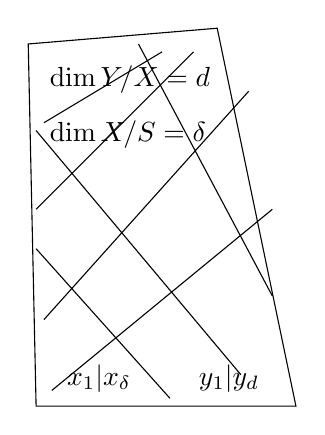
\begin{tikzpicture}[x=1cm,y=1cm]
\draw (0,4.6)--(2.4,4.8)--(3.4,0)--(0.1,0)--cycle;
\node[anchor=west] at (.15,4.15) {$\dim Y/X=d$};
\node[anchor=west] at (.15,3.45) {$\dim X/S=\delta$};
\node at (.9,.35) {$x_1\text{—}x_\delta$};\node at (2.55,.35) {$y_1\text{—}y_d$};
\draw (.2,3.6)--(1.7,4.5) (.1,2.5)--(2.1,4.5) (.2,1.1)--(2.8,4) (.3,.2)--(3.1,2.5) (.1,3.5)--(2.7,.4) (.1,2)--(1.8,.1) (1.4,4.6)--(3.1,1.4);
\end{tikzpicture}}}}

\uline{\S1} Descente \inserted{d'objets plats} par morphismes quelconques

\uline{\S2} Descente d'objets quelconques par morphismes plats.
\margin{\unsure{intervertir}}

\uline{\S3} Application \inserted{de \S1} aux morphismes non ramifiés

\uline{\S4} Cas particuliers élémentaires : Espaces $X/G$, descente galoisienne non ramifiée, le \uline{contre-exemple de Nagata}. Interprétation de la descente plate finie par \uline{opérateurs quasi-différentiels}. Cas de Cartier.
\margin{\uline{\unsure{Conditions de descente}} \uline{\unsure{d'une famille}} \unsure{de schémas} \uline{\unsure{projectifs ?}} \uline{Pas ici le lieu !}}
\margin{Les théorèmes \unsure{vus au} \S1 \unsure{ne sont pas utilisés au} \S\unsure{7}.}
\margin{\S1 à 7}

\uline{\S5} $\underline{\operatorname{Hom}}_S(X,Y)$ et $f_*(X)$ : formalisme général, cas d'existence pour $X$ fini et plat sur $S$. [Est lié à la \unsure{technique|théorie} de la descente \deleted{seulement} par deux endroits

a) Existence de \uline{Hom} si $X\to S$ est \unsure{géom. projectif} -- fini et plat --

b) Relations entre l'existence de $f_*(X)$, $\underline{\operatorname{Hom}}_S(X,Y)$, et la possibilité de descente.] Cas particuliers : $\unsure{\check V(\mathcal F)}$ etc.
\margin{\unsure{Propriétés diverses de permanence}}

\uline{\S6} Application des schémas \uline{Hom} : la géométrie différentielle, les Picard, Greenberg d'égale caractéristique etc

\uline{\S7} \unsure{Hyperproblèmes|Hyperschémas} sur $S$. Critères de représentabilité.

[y inclure aussi le critère général d'existence par théorie des modules formelle]
\margin{\uline{ailleurs ?} Ne vient ici que par l'utilisation dans \unsure{ce qui suit} de l'existence de $\unsure{f_*}$. Pourrait venir \unsure{entièrement} dans Ch. \uline{IV}, mais \unsure{obligerait} d'y développer \unsure{longuement} des \uline{Hom}.}

\uline{\S8} \unsure{4} \deleted{\unsure{Cas particuliers}} \inserted{Théorèmes} \uline{fondamentaux d'existence}

A) Théorie formelle des modules. Extension des solutions\ldots

\uline{\S9} \deleted{B) \unsure{2}} $f_*(X)$ si $X$ est projectif sur $Y$, $Y$ plat et propre sur $S$.

\uline{\S10} C) Picard.
\margin{\unsure{ensemble ?}}

[Critères de simplicité, de propreté, de platitude ?]
% archive foliation: 36

\scanpage{38}
\uline{Proposition} Soit $f:T\to S$ un morphisme fini localement libre, et soit \deleted{$\unsure{\mathcal F}$} $F$ un faisceau qu. coh. localement libre sur $T$, de sorte que $f_*(F)$ est un faisceau \inserted{qu. coh.} localement libre sur $S$. Alors on a un isomorphisme fonctoriel
\[
\boxed{f_*(\underline{\check V}(F))=\underline{\check V}(f_*(F))}
\]
[Cet isomorphisme est compatible aux images inverses, \inserted{en particulier} \unsure{localisations|localisation}].
% archive foliation: 37

\scanpage{39}
\diagram{\begin{tikzcd}X\arrow[d,"f"]\\Y=\operatorname{Spec}(\mathcal O)\end{tikzcd}}
\[
F=\widetilde M
\]
$f$ \inserted{plat et} propre, $Y$ schéma noethérien local, $F$ cohérent sur $Y$.
\[
F'=f^*(F),\qquad F'_1\subset F'
\]
\inserted{ss faisceau cohérent.}
\deleted{\unsure{on}} Je dis qu'il y a un plus \unsure{petit|grand} ss-faisceau cohérent $F_1$ de $\unsure{F'|F}$ t.q. $f^*(F_1)\supset F'_1$.

Si $f^*(F_1)$ et $f^*(F_2)\supset F'_1$ alors
\[
f^*(F_1\cap F_2)=f^*(F_1)\cap f^*(F_2)\supset F'_1
\]
\margin{platitude de $f$}
$F_i\subset F$ tq $f^*(F_i)\supset F'_1$ \deleted{\unsure{forment}} \unsure{une famille filtrante décroissante}. Il reste à prouver que $F_1=\bigcap F_i$, alors $f^*(F_1)\supset F'_1$ i.e. l'image de $F'_1$ dans $F'/f^*(F_1)=f^*(F/F_1)$ est nulle. Remplaçant $F$ par $F/F_1$, on est ramené à prouver ceci : \uline{si} $\bigcap F_i=0$, \uline{alors} \deleted{$\bigcap\unsure{f^*(F_i)}=0$} \inserted{tout faisceau cohérent $F'_1$ contenu dans $\bigcap f^*(F_i)$ est nul} [$f$ propre \deleted{\unsure{complet|surjectif}}, les $F_i$ filtrants décr. dans $F$ cohérent, $Y$ local et complet].
\margin{[\unsure{on sait même que} $\bigcap f^*(F_i)$ est nul ?]}
\deleted{Comme $F'_1=\bigcap\unsure{f^*(F_i)}$ \unsure{de}}
\deleted{Soit $s$ une section de}

$F'_1$ est fermé, il suffit de prouver qu'il ne rencontre pas $f^{-1}(y)$ ($y$ le pt fermé de $Y$) donc de prouver que si $s$ est une section de $F'_1$ sur un ouvert $U$, elle est nulle en $\forall\ x\in f^{-1}(y)$. Or comme $\bigcap M_i=0$, les $M_i$ tendent vers $0$ dans $M$ (?)

\margin{N.B. Faut définir \unsure{pour un} $\mathcal O$-module $M$, les $F_i$ par des $M_i\subset M$, pour \uline{\unsure{définition}} \unsure{en vrai sens}, $\unsure{\bigcap_iF_i}=\widetilde{\bigcap M_i}$ (ce n'est pas le faisceau $\bigcap$, mais \unsure{l'inf dans les faisceaux qu. coh.}).}
\margin{Énoncé : sous conditions envisagées ($f$ propre, les $F_i$ décroissants dans $F$ cohérent, $Y$ local et complet), $f^*(\bigcap F_i)=\bigcap f^*(F_i)$ ?}
\margin{\uline{\unsure{Arranger les notations}}}
% archive foliation: 38

\scanpage{40}
% archive foliation: 39
\diagram{\begin{tikzcd}
& X \arrow[d] & X\times_S S' \arrow[ul] \arrow[d] \\
S & T \arrow[l,"f"'] & \\
\unsure{S'|Z'} \arrow[uu] & S'\times_S T=T' \arrow[l] \arrow[u] \arrow[uur,dashed,bend right] &
\end{tikzcd}}
\diagram{\begin{tikzcd}
& X_s \arrow[d] & X'_{s'} \arrow[ul] \arrow[d] \\
s \arrow[r,dash] & T_s & \\
s' \arrow[r,dash] & T'_{s'} \arrow[u] \arrow[uur,dashed,bend right] &
\end{tikzcd}}
\figure{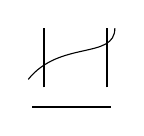
\begin{tikzpicture}[scale=.5]\draw (0,0)--(0,1.5);\draw (1.6,0)--(1.6,1.5);\draw (-.4,.2) .. controls (.4,1.2) and (1.8,.7) .. (1.8,1.5);\draw(-.3,-.5)--(1.7,-.5);\end{tikzpicture}}
\uline{Proposition 2} Supposons que $f_*(X/T)$ existe, et que pour tt $s\in S$, \deleted{toute} multisection de $X_s/T_s$ définie sur une extension finie \inserted{$k'$} [quelc] de $k(s)$, soit ``contenue'' dans un ouvert \deleted{\unsure{affine relatif|affine}} $U_i\otimes k'$ ($U_i$, \unsure{famille d'ouverts donnée|famille donnée}). Alors $f_*(X/T)$ est réunion des $f_{i*}(U_i/T)$ ($\unsure{f_i=f(U_i)|f_i=f\vert U_i}$).
\margin{\unsure{de finité}}
[On suppose $T$ et $X$ de type fini sur $S$]

En effet, \deleted{\unsure{on}} il suffit de montrer pour \deleted{\unsure{tout}} pt \deleted{fermé} de $f_*(X/T)$ que \unsure{$\exists i:\ \in f_{i*}(U_i/T)$}.
Un tel pt fermé est défini par un corps $K$ sur un $k(s)$, et une \inserted{multi}section définie sur $K$ de $X_s$ sur $T_s$. On peut le supposer \deleted{défini sur un} $K$ fini sur $k(s)$, à cause des hyp. de finitude \unsure{faites dans le|posées dans le} \deleted{\illegible{1}} premier cas. Il provient donc \unsure{---}.

\margin{\unsure{complète prop. 2}}
\deleted{\uuline{Corollaire}} \inserted{\uline{Proposition $2^{bis}$}} Supposons que les \inserted{multi}sections $X_s/T_s$ définies sur une extension finie (ou p. \unsure{quelconque}) $k'$ de $k(s)$ soient contenues dans un ouvert \deleted{\uline{affine}} \deleted{\unsure{relatif}} \inserted{d'}une famille $U_i$.
Supposons que les $f_{i*}(U_i/T)$ existent, alors il en est de $=$ de $f_*(X/T)$.

\scanpage{41}
% archive foliation: 40
Démonstration. On \deleted{\unsure{considère}} sait que $f_*(U_{ij}/T)$ existe aussi, il s'envoie par imm. ouverte dans les $f_*(U_i)$ et $f_*(U_j)$. Les conditions de cohérence se \unsure{vérifient}, d'où un préschéma $\uline{H}$ sur $S$, \deleted{\unsure{les}} réunion d'ouverts $H_i\simeq f_*(U_i/T)$.
On définit par recollement un $T$-hom
\[
H\times_S T\longrightarrow X,
\]
\inserted{$\unsure{\text{induit par}}\ H_i\times T\longrightarrow U_i$.}
puis on doit montrer que \deleted{\unsure{H=}} $f_*(X/T)$.
\margin{Pour éviter nos difficultés \unsure{pour $H_i$ est le plus gd ss-ouv de $H$|que $H_i$ est le plus gd ss-ouv de $H$} \deleted{\unsure{contenu}} \unsure{dont l'image} $\unsure{\xi_i^{-1}|\xi_i\to1}$ \unsure{ouvert en} $H\times_S T$ \unsure{est le} \unsure{$\varphi^{-1}(U_i)$} \unsure{de $\varphi$}.}
\deleted{$S'\longrightarrow\unsure{H|S}$ \unsure{sur $S$}, \unsure{quelconque},} \inserted{sur $S$, il faut montrer} que
\[
\operatorname{Hom}_S(S',H)\xrightarrow{\sim}\operatorname{Hom}_T(S'\times_S T,X).
\]
On peut supposer $S=S'$.
\deleted{\unsure{Il y a} \uline{injection}, car si \deleted{\unsure{on a}} \inserted{deux} \deleted{\unsure{hom}} \deleted{\unsure{homomorphismes}} sections \deleted{$\unsure{S,S'}$} $u,v:S\longrightarrow H$ \deleted{$\unsure{S}\longrightarrow T$}, définissent le $=$ \deleted{\unsure{section}} \inserted{homomorph.} $T\longrightarrow X$, les images inverses $T_i$ par ce dernier \deleted{\unsure{des ouverts}} des $U_i$ \uline{recouvrent} $T$,}
\deleted{\diagram{\begin{tikzcd}
\unsure{S} \arrow[r] \arrow[d] & \unsure{H} \arrow[d] \\
\unsure{S\times T} \arrow[r] & \unsure{U_i}
\end{tikzcd}}}
\diagram{\begin{tikzcd}
& X \arrow[d] & \\
S & T \arrow[l] & \\
H \arrow[u] & H\times_S T=\bigcup H_i\times_S T \arrow[l] \arrow[u] \arrow[uu,bend right] &
\end{tikzcd}}
i.e. il faut que
\[
\operatorname{Hom}_S(S,H)\simeq\operatorname{Hom}_T(T,X).
\]
Soit $\varphi$ une section de $X/T$,

\scanpage{42}
% archive foliation: 41
D'après l'hypothèse \deleted{les $\varphi^{-1}(U_i)$ \uline{recouvrent} $T$,} pour tt $s\in S$, il existe un $i(s)$ tel que $\varphi(T_s)\subset U_{i(s)}$. Il est évident (préciser) que l'on peut trouver un voisinage $V_{(s)}$ de $s$ tel que $\varphi(T\vert V_{(s)})\subset U_i$. On en déduit un hom $V_{(s)}\longrightarrow H_i$, d'où $V_{(s)}\longrightarrow H$.
Je dois montrer que ça se recolle. C'est \unsure{strictement formel} ---.

\uline{Théorème} On suppose $T$ fini et loc. libre sur $S$,
\deleted{et $X/S$ quelconque. Pour que \unsure{$\operatorname{Hom}$}}
On suppose de plus que \deleted{\unsure{l'on ait dans}} \deleted{l'une des deux conditions suivantes\par (i) $T\longrightarrow S$ est \unsure{univ. injectif|purement injectif}\par (ii)}
Pour tout $\unsure{t\in S|s\in S}$, tt multisection de $X_s$ sur $T_s$, définie sur une extension finie de $k(s)$, soit contenue dans un ouvert affine de $X$.
\margin{$k(s)\qquad k(t)$}
\deleted{[\unsure{condition Hyp.}} \inserted{Alors} \deleted{\unsure{enfin si tt partie}}
$f_*(X/T)$ existe, et est réunion des $f_{i*}(U_i/T)$, où $U_i$ parcourent ts ouverts affines de $X$.

\scanpage{43}
% archive foliation: 42
\uline{Cor. 1} La dernière hyp. du \unsure{précédent énoncé|th. précédent} est vérifiée dans chacun des deux cas suivants

(i) $T/S$ est \unsure{purement injectif|purement inséparable}

(ii) $S=\bigcup S_i$ ($S_i$ ouverts), tels que tt \inserted{partie finie de} $X\vert S_i$ soit contenue dans un ouvert affine.
[p. ex. $X$ quasiproj. sur $S$].

\uline{Cor. 2} Sous les conditions dites, soit $X'$ un ss-schéma fermé de $X$, \inserted{\unsure{soit} $f'=f\vert X'$.} Alors $f'_*(X')$ existe, et est un ss-schéma \uline{fermé} de $f_*(X)$.

\scanpage{44}
% archive foliation: 43
\diagram{\begin{tikzcd}&X\arrow[d]\\S&T\arrow[l,"f"']\end{tikzcd}}
$f_*(X/T)$ \qquad $T$ fini sur $S$
\diagram{\begin{array}{llll}
\text{Si}&X/T\text{ est affine},&f_*(X/T)\text{ aussi}.&\\
\text{si}&\text{---}\left\{\begin{array}{l}\text{projectif}\text{ +}\\\text{propre}\end{array}\right.&\text{---}&\left.\vphantom{\begin{array}{l}1\\2\end{array}}\right\}\ \uline{\text{pourvu que}}\ f\ \uline{\text{séparable}}\ (*)\\
\text{si}&\text{quasi-projectif},&\text{---}&
\end{array}}
\margin{\unsure{donner un énoncé} ``général'' \unsure{dans le cas}: \unsure{$f$ plat|$f$ fidèle}.}

Lemme $f_*$ est exact à gauche, \deleted{\unsure{vérifie que le produit}} \inserted{en particulier}
\[
f_*(T/T)=S,\quad f_*(X\times_T Y/T)=f_*(X/T)\times_S f_*(Y/T),\quad f_*(X\times_Z Y/T)=f_*(X/T)\times_{f_*(Z/T)}f_*(Y/T).
\]
Le foncteur $f_*$ transforme imm. ouvertes en imm. \deleted{\unsure{fermées}} \inserted{ouvertes} et \unsure{l'on a une hyp. qui assure}, \deleted{[\unsure{pourvu que}} \inserted{\unsure{finies}}
\[
f_*(X/T)=\bigcup_i f_*(U_i/T),\quad\text{où les }U_i\text{ recouvrent }X]
\]
imm. fermées en imm. fermées. \deleted{\unsure{Les}} \deleted{\unsure{autres assertions},}
[N.B. cette assertion doit pouvoir être \unsure{déduite|établie} par la technique de descente].
\inserted{\unsure{que le $\subset$ visé est même l'assertion;}}

\margin{(*) Se voit par descente:\par
Si $Y/S$ est tel que $f^*(Y)/S'$ soit propre resp. projectif, alors $Y/S$ l'est [Dans le deuxième cas, on suppose $T/S$ fini et plat sur $S$ \uline{loc. noeth.} \deleted{\unsure{(1)}}\par
(i) \unsure{faire détail dans le cas actuel} pour voir l'assertion, en se ramenant au projectif type, \deleted{\illegible{2}} travaillant sur $\uline{\mathbf Z}$ et de \unsure{finiture}, il faut prouver ceci:\par
Si un faisceau loc. libre inversible $\uline{L}$ sur $X$ est $T$-ample, alors $f_*(\uline{L})$ [qui est un faisceau loc. libre de rang $d$ sur $f_*(X/T)$ est tel que $\det f_*(\uline{L})$ est $S$-ample --\par
Dans le premier cas, on utilise le lemme de Chow, en notant que si $X'\longrightarrow X$ est surjectif, alors $f_*(X')\longrightarrow f_*(X)$ l'est -- \deleted{\illegible{2}}, on peut pour cela supposer $S=(\operatorname{spec} k)$; et \unsure{préciser par descente} ---\par
Ici il faut $S$ \deleted{\unsure{noeth.}} \inserted{loc.} noeth.\par
\uline{Question} Si $T/S$ est fidèlement plat non fini, et $\unsure{X/S|Y/S}$ est tel que $Y\times_S T/T$ soit propre, est-il vrai que $Y/S$ l'est? -- Oui dans le cas $S$ loc. noeth., car on utilise encore le lemme de Chow.}

De $=$, $f_*$ transforme \deleted{\unsure{applications}} morphismes affines en morphismes affines [en effet, soit $\varphi:X\longrightarrow Y$ affine, \deleted{alors} on est ramené \inserted{par recollement} au cas où $Y$ est affine et $X\subset Y\deleted{\unsure{\otimes_T}} Z\deleted{\unsure{\subset X}}$ est schéma fermé \inserted{$Z/T$ affine}, on se ramène au cas $\unsure{X\supset Y\otimes_T Z|X=Y\otimes_T Z}$ puis on tient des imm. fermées] il transforme morphismes projectifs en morphismes projectifs si $T/S$ est séparable, et en tous cas il transforme morphismes quasi-projectifs en morphismes quasi-projectifs.

[Méthode, du moins si $Y$ est noeth. \inserted{si on $X_T\longrightarrow Y/T$} \deleted{\unsure{du}} qu. proj. de type fini sur $T$ donc un faisceau coh. sur $Y$ est quotient d'une puissance de $T$; $U$ ouvert connexe, et il est plus précis de pouvoir assurer que l'on

\scanpage{45}
% archive foliation: 44
prenne le det du faisceau descendu, on trouve à partir d'un faisceau \unsure{très ample|rel. ample} sur $X/Y$, un faisceau ample sur $f_*(X/T)/f_*(Y/T)$ \deleted{\unsure{etc}}]. Kif-kif pour propre.

\uline{Proposition} Soit $g:X/T\longrightarrow Y/T$ un morphisme, et soit $\uline{L}$ un faisceau inversible sur $X$ \uline{ample} \deleted{pour} (resp. très ample) pour $g$. Alors $\det f_*(\uline{L})$ est un faisceau ample (resp. très ample) pour
\[
f_*(X/T)\longrightarrow f_*(Y/T)
\]
Démonstration. \unsure{(2)} On peut supposer $Y$ affine, l'amplitude \deleted{\unsure{est un caractère}} étant une notion locale. \unsure{(1)} On \deleted{\unsure{est ramené}} \inserted{est ramené au cas ``ample''.} \deleted{\unsure{que ce résultat}} De plus, on est ramené à prouver ceci: Si $X=\mathbf P_Y^n$, et $\uline{L}$ le faisceau fondamental dessus, alors $f_*(\uline{L}/T)$ \deleted{est} définit une immersion projective fermée de $f_*(\mathbf P_Y^n)$ sur \unsure{ce qui est} $f_*(Y/T)$. Mais utilisant la commutation de $f_*$ aux \unsure{chg. de base|produits}, on est ramené au cas où $Y=T$. De plus, la question étant locale, on peut supposer $S$ affine $=\operatorname{Spec}(A)$, $T=\operatorname{Spec}(B)$, $B$ étant libre de type fini (rang $d$) sur $A$.
\margin{\unsure{Sur le réseau fidèle|Sur le réseau fini}}
\margin{$\unsure{f_*(U/T)\longrightarrow f_*(X/T)}$}
\margin{$S\qquad T$}
\margin{\deleted{N.B. \unsure{Rien de si simple|Rien de plus simple} si on introduit sur $Y$ le foncteur $f_*(\uline{L})$ (qui \unsure{n'est pas de} type fini en général) pour \uline{prouver} \unsure{que le faisceau} \unsure{constitue l'imm. projective}, \unsure{on trouve les} \unsure{sections} \unsure{en nombre} \unsure{fini}. \unsure{Donc pour} \uline{tt} faisceau coh. \unsure{(quasi-cohérent)}}}

On est ramené \deleted{\unsure{en}} à deux vérifications:

A) Détermination de la grassmannienne.
et d'un faisceau ample dessus, i.e. d'une \inserted{immersion projective de la dite.}

\scanpage{46}
% archive foliation: 45
B) Étude de la situation suivante: On a un préschéma $G$ [la grassmannienne en question] un faisceau loc. libre de rang $d$ d'algèbres $\uline{A}$ sur $G$ (l'image inverse de $f_*(\mathcal O_T)$] un faisceau loc. libre de $\uline{A}$-\deleted{\unsure{alg.}}-modules $\uline{F}$, un sous-faisceau de $\uline{\mathcal O}_G$-\deleted{\unsure{alg.}} modules $\uline{F}_1$, \inserted{tel que $\uline{F}/F_1$ soit} loc. libre de corang $kd$.
On s'intéresse, pour tt préschém. $G'$ sur $G$, [non $G\times_S S'$] de savoir si \deleted{$\uline{F}'_1\subset\uline{F}'$ est un $\unsure{B}$-module} \inserted{$\unsure{F'_1/\uline{F}'|\uline{F}'/F'_1}$ est loc. libre de} \deleted{\unsure{de}} rang $k$ \uline{sur $\uline{A}'$}. On veut définir un ss-schéma \deleted{fermé} $G_*$ de $G$ tel que la cond. néc. et suffis. cherchée soit que $G'\longrightarrow G$ se factorise par $G_*$.

La \deleted{condition} \inserted{question} est \uline{locale} sur $G'$ (détermination de la représentabilité d'un foncteur!), on peut supposer: \deleted{$\unsure{\uline{E}=\uline{A}^n},\ \uline{F}_1=$}

(i) $G$ affine d'anneau $A$

(ii) $\uline{A}$ définie par une $A$-algèbre $B$ ayant une base $b_1,\ldots,b_d$

(iii) $\uline{F}$ défini par $B^n$, donc a une base $b_\alpha^{(i)}$ $(1\leq i\leq n,\ 1\leq\alpha\leq d)$

(iv) $\uline{F}_1$ a une base \deleted{$\unsure{b'_i}$} $(e_\gamma)_{\unsure{1\leq i\leq(n-k)d|1\leq\gamma\leq(n-k)d}}$, qu'on complète en une base d'un supplémentaire $(d_j)_{1\leq j\leq kd}$

On se donne \deleted{\unsure{la}} \inserted{une} condition néc. et suffisante

\scanpage{47}
% archive foliation: 46
pour que $F_1$ ait les propriétés dites. \deleted{\illegible{2}}

$1^\circ)$ $\uline{F}_1$ doit être stable par multiplication par $\uline{B}$, i.e. \deleted{\unsure{que}} les composantes de $b_i e_\lambda$ suivant les $d_\mu$, soient $\varphi_{i\lambda\mu}\in A$, doivent être \uline{nulles}. D'où des \uline{équations}
\[
\varphi_{i\lambda\mu}=0\qquad\left[\begin{array}{l}
1\leq i\leq d\\
1\leq\lambda\leq(n-k)d\\
1\leq\mu\leq kd
\end{array}\right]
\]
\margin{Soit $G_1$ le sous schéma de $G$ défini par ces équations. On est ramené au cas ---}

$2^\circ)$ Le $B$-module quotient \deleted{$\unsure{F_1/F|M=B^k}$} $F/F_1=M$ est projectif de rang $\unsure{k|n}$. Il a une base sur $A$ de la forme $(m_i)_{1\leq i\leq kd}$,
Soient $\xi=(\xi_1-\xi_k)$ \deleted{\unsure{des}} \inserted{une suite de $k$} \unsure{éléments} de $M$. Pour qu'ils forment une base sur $B$, il f. et s. que $B^k\xrightarrow{u_\xi}M$ défini \deleted{\unsure{soit}} bijectif. Or deux $B^k$ et $M$ ont des bases, donc on peut former $\det(u_\xi)$, la condition est que $\det(u_\xi)$ soit inversible. \deleted{Donc pour que} Pour que en un pt $x\in\operatorname{Spec}(A)$, $M_x$ soit libre sur $B_x$, il faut et il suffit qu'il existe $\xi\in(M_x)^k$ tel que $\det(u_\xi)$ soit inversible dans $A_x$. On voit facilement que l'on peut aussi prendre les $\xi\in M^k$. Donc pour tt \deleted{\unsure{un}} $\xi\in M^k$, soit $U_\xi$ l'ouvert \deleted{\unsure{par}} des non-zéros de $\det(u_\xi)$. Soit $U=\bigcup U_\xi$. C'est
\margin{\unsure{préciser un th., en complétant|préciser un peu, en complétant} \unsure{tenant compte des conditions de validation encore}}

\scanpage{48}
% archive foliation: 47
l'ouvert cherché [N.B. la locale liberté de $M$ en $x$ est en effet une condition \uline{ponctuelle} et de nature locale, \deleted{\unsure{reste}} compatible avec l'extension des corps de base $k(x)$ ---]
\figure{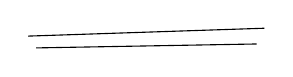
\begin{tikzpicture}\draw(0,0)--(3,.1);\draw(.1,-.15)--(2.9,-.1);\end{tikzpicture}}
Sous les \unsure{réserves|conditions} habituelles, \uline{si} $g:X/T\longrightarrow Y/T$ \uline{est de type fini}, \uline{alors} $f_*(g)$ \uline{est de type fini}.
[$S$ est \uline{loc. noeth.})
On est ramené au cas où $Y=T$, \deleted{$X$ affine} \inserted{Par} \deleted{sur $T$. On peut donc supposer} hypothèse, \deleted{\unsure{toute}} multisection d'un $X_s$ sur un $T_s$ est contenue dans un ouvert \deleted{\unsure{aff.}} \inserted{affine $U$}.
\unsure{Prouvons|Prenons} qu'un nb fini de tels ouverts affines \deleted{\unsure{X}} suffisent. \deleted{On peut supposer} \inserted{Soit en effet} \deleted{$S$ affine, dans le cas}
\[
\unsure{X^\nu}=\underbrace{X\times_S\cdots\times_S X}_{\nu},
\]
pour tt ouvert affine $U$ de $X$, soit
\[
U^\nu=\underbrace{U\times_S\cdots\times_S U}_{\nu},
\]
$U^\nu$ est un ouvert de $X^\nu$. \deleted{\unsure{Pour voir}} \inserted{Comme} $X^\nu$ est \deleted{\unsure{quasi}} noethérien, il existe un nb \uline{fini} d'ouverts affines $U_i$ tels que
\[
\bigcup U_i^\nu=\bigcup U^\nu.
\]
Soient $(x_1,\ldots,x_\nu)\deleted{\in\unsure{(X_s)^\nu}\ \unsure{pris dans un même ouvert affine}}$ \deleted{$U$. Alors} soit $x\in X^\nu$ de projections les $x_i$. Alors les $x_i$ sont dans un ouvert affine
\margin{\uuline{\unsure{rédiger convenablement}}}

\scanpage{49}
% archive foliation: 48
$U$ sss $x\in U^\nu$, \deleted{donc} \unsure{or ceci implique} $x\in U_i^\nu$ pour $i$ convenable i.e. les $x_\alpha\in U_i$. \unsure{O.K.}

On est ainsi ramené au cas où $X$ est \uline{affine} sur $Y$. Mais alors, on est $=$ ramené au cas où $X=\unsure{\operatorname{Sym}|\operatorname{Spec}}(\unsure{\uline F})$, où $F$ est un faisceau loc. libre de rang $n$ sur $T$. On sait qu'alors
\[
f_*(X/T)=\unsure{\operatorname{Sym}|\operatorname{Spec}}(f_*\unsure{\check F|\uline F}).
\]

\deleted{\uline{\unsure{Corollaire}} $\unsure{f_*}$ \unsure{de}}

\uline{Remarque} Il n'est pas vrai en général que la dim. des fibres de $f_*(X/T)/S$ soit majorée par $d$ fois la dim des fibres de \deleted{$\unsure{f_*}$} $X/T$. Ex:
$S=\operatorname{Spec}(k)$, $T$\deleted{$=\operatorname{Spec}k[\varepsilon]/\unsure{\varepsilon^2}$} est purement radiciel sur $S$, $X=T\times_S T$ i.e. $f_*(X/T)=\uline{\operatorname{Hom}}_S(T,T)$. Ce dernier peut être de \uline{dim} \inserted{$>0$} \deleted{$\unsure{d}$} sur $k$. Exemple: le groupe des automorphismes de la $k$-algèbre $\unsure{A|k}$ est de dim $>0$.
\margin{\unsure{voir précisé|voir préciser} plus bas}

\scanpage{50}
% archive foliation: 49
\diagram{
\begin{tikzcd}
f_*(X/T) \arrow[r] & f_*(Y/T) \\
S'_1 \arrow[u] \arrow[r,hook] & S' \arrow[u] \arrow[ul,dashed]
\end{tikzcd}\qquad (A)
}
\diagram{
\begin{tikzcd}
& T \arrow[dl] & & Y \\
S & & T' \arrow[ul] \arrow[dl] \arrow[ur] \arrow[r,dashed] & X \arrow[u] \\
& S' \arrow[ul] & & T'_1 \arrow[ul,hook] \arrow[u] \arrow[dl] \\
& & S'_1 \arrow[ul]
\end{tikzcd}\qquad (B)
}
\diagram{\begin{tikzcd}T'_1 & T'\end{tikzcd}}

\deleted{\uline{Proposition}} $\{$\uuline{Théorème?}$\}$ $T$ \deleted{\unsure{fini et plat} sur $S$ loc. noeth.} \inserted{sur $S$ (\unsure{pas néc. fini\ldots})} $*$

$X/T\xrightarrow{g}Y/T$ un morphisme \deleted{\uline{simple}} \inserted{de type fini} de $T$-préschémas.

On suppose que $f_*(X/T)$ et $f_*(Y/T)$ existent et \deleted{loc. noethériens} \inserted{loc. de type fini sur $S$}, \deleted{\unsure{que} $f_*(X/T)\unsure{\longrightarrow|,}f_*(Y/T)$ est de type fini}, et que \inserted{$S$ et} $T$ sont loc. noeth.
\margin{$2.\ \longrightarrow$}
\inserted{(i) \unsure{Supposons} $T/S$ \unsure{affine}.}

Si $X/T\xrightarrow{g}Y/T$ est simple, il en est de $=$ de $f_*(g)$.

\deleted{Il faut}

(ii) Supposons $T/S$ \deleted{\unsure{fini}.} \inserted{de type fini}, si $g$ est \uline{étale}, $f_*(g)$ est étale.

Démonstration. (i) Il faut pouvoir compléter le diagramme (A) par une flèche oblique, \deleted{\unsure{de} $S$} quand $\unsure{S'|S'_1}$ est affine, \inserted{et de type fini sur $S$}, $S'_1$ un ss-schéma fermé ayant $=$ schéma réduit.
\margin{On peut supposer $S$ affine}

Cela revient à compléter de façon analogue le diagramme (B). C'est possible, car $T$ \unsure{étant} affine, $T'$ le sera aussi, et $T'_1\to T'$ sera une immersion fermée définissant un isom. de $T'_1$ sur un ss-schéma fermé de $T'$ ayant $=$ ss-schéma \unsure{réduit}, \unsure{par} \illegible{1}.

\scanpage{51}
% archive foliation: 50
(ii) Ce raisonnement vaut aussi sans supposer $T/S$ affine, si $g$ est \uline{étale}, \deleted{\unsure{car}} Ainsi, $f_*(g)$ sera simple. Pour prouver qu'il est étale, il suffit de prouver que ses \uline{fibres sont} \deleted{\unsure{de}} \inserted{finies} \deleted{dim $0$ (\unsure{uniformément})}. \inserted{(\unsure{uniformes})} On est ramené au cas où $S=\operatorname{Spec}(k)$, $k$ un corps, et à prouver que si $k'$ est une clôture algébrique de $k$, alors il n'y a qu'un nb fini de $k'$-pts de $f_*(X)$ au dessus d'un $k'$-point de $f_*(Y)$, i.e. qu'il n'y a qu'un nb fini de sections de $X'/T'$ qui relèvent une section donnée de $Y'/T'$.
\margin{\unsure{donner un} \uline{\unsure{contre-ex.}} \unsure{non fini}}
\diagram{\begin{tikzcd}&X \arrow[r]&Y\\ k&T\end{tikzcd}}
\diagram{\begin{tikzcd}&f_*(X)\arrow[d]\\\operatorname{Spec}(k')\arrow[r]&f_*(Y)\end{tikzcd}}

[$\unsure{\text{où}}$ $'$ désigne ext. des scalaires de $k$ à $k'$]
Or $T'$ sera noethérien [de type fini sur $k'$] donc n'a qu'un nb fini de comp. connexes. On peut supposer $T'$ connexe. Mais le relèvement est connu dès qu'on connaît l'image d'un pt. On \unsure{trouve|aura} donc

\uline{Corollaire} 1 Soit $\nu$ le maximum des nbs \deleted{\unsure{resp.}} de composantes connexes absolues des $T_s$ ($s\in S$), et soit de $=$ $n$ le maximum analogue pour $X/Y$. Alors le maximum

\scanpage{52}
% archive foliation: 51
analogue pour $f_*(X/T)\to f_*(Y/T)$ est $\leq n^\nu$.

\deleted{\uline{\unsure{Corollaire 2}}}
\deleted{
\uline{Complément} Soit \deleted{\unsure{$T/S$ fini}\illegible{2}} \inserted{[si $T/S$ est \deleted{affine} fini]}
\unsure{Soit}
\[
d=\sup_{y\in Y}\dim g^{-1}(y),\quad\text{et}\quad
d'=\sup_{\bar y\in f_*(X/T)}\dim f_*(g)^{-1}(\bar y).
\]
\inserted{Soit $n=\deg(T/S)$}
Alors on a $d'\unsure{\leq|=}nd$.

On a égalité si ttes les fibres \unsure{géom.} \unsure{égales à $\nu$} \unsure{et} $\deg_{\mathrm{sép}}(T/S,s)$ est indépendant de $S$ (donc égal à $\nu$), si les fibres de $\unsure{f|g}$ ont ttes $=$ dimension $d$ en \unsure{tt. leurs pts}, il en est de $=$ \unsure{de}.
}

\uline{Corollaire 2} Supposons $T/S$ fini de degré $n$ \unsure{f. plat|plat}.
Supposons qu'on est sous les conditions (i).
Soit \deleted{\unsure{donc}} $s\in S$, soit $D(s)$ l'ens. des dimensions des \deleted{fibres} comp. des fibres de $X_s\to Y_s$; \deleted{\unsure{de}} soit $D'(s)$ l'ens. analogue pour $f_*(X/T)_s\to f_*(Y/T)_s$. Alors $D(s)=nD'(s)$.
\diagram{\begin{tikzcd}&X_s\arrow[r]&Y_s\\k(s)&T_s\end{tikzcd}}
En particulier, si ttes les composantes de ttes les fibres de $g$ ont $=$ dimension $d$, \inserted{\unsure{alors}} ttes les composantes de ttes les fibres de $f_*(g)$ ont $=$ dimension $nd$.

\scanpage{53}
% archive foliation: 52
\uline{Dém} On peut supposer $S=\operatorname{Spec}(k)$, De plus, on peut supposer $k$ alg. clos. Enfin, d'après
\[
(\coprod f_i)_*(X/T)=\prod_i f_{i*}(X_i/T_i),
\]
on est ramené au cas où $T$ est connexe, i.e. $T\to S$ géométriquement injectif. On peut alors supposer $X$ et $Y$ affines, et $X\xrightarrow{g}Y$ \deleted{\unsure{un}} se factorisant en
\diagram{\begin{tikzcd}X\arrow[r,"{\inserted{g_1}}","{\deleted{\unsure{g_2}}}"']&Y[t_1,-,t_d]\arrow[r,"g_2"]&\unsure{Y'|Y}\end{tikzcd}}
\deleted{\diagram{\begin{tikzcd}X\arrow[r]&Y\end{tikzcd}}}
où $g_1$ est étale et $g_2$ la projection can.
\deleted{\unsure{D'} $f_*(g)=f_*(g_2)f_*(g_1)$, et $f_*(\unsure{g_2|g_1})$ étant étale,} \deleted{\unsure{et}} Il faut prouver que ttes les fibres de $f_*(g)$ ont dim $nd$.
Comme $f_*(g)=f_*(g_2)f_*(g_1)$, \inserted{et $f_*(\unsure{g_2|g_1})$ est étale} on est ramené au cas où
\[
X=Y[t_1,-,t_d]=Y\times_T\unsure{\mathbf Z|T}[t_1,-,t_d]
\]
\deleted{\unsure{où} $\unsure{Z|2}=T[t$}
On est ramené (formule de produits): prouver que les fibres de
\[
f_*(T[t_1,-,t_d]/T)
\]
sont de dim $nd$, ce qui est trivial.

\scanpage{54}
% archive foliation: 53
\diagram{\begin{tikzcd}&X_s\arrow[r]&Y_s\\k(s)=k&T_s\end{tikzcd}}
\diagram{\begin{tikzcd}&X'_s\arrow[r,dash]&Y'_s\\k'&T'_s\arrow[u]\arrow[ur]\end{tikzcd}}
\margin{Nb de comp. connexes absolues de $T_s$: $\nu_s$
\[
\nu=\sup\nu_s\qquad
\left\{\begin{array}{l}n=\deg T/S\\d=\dim.\ \text{fibres de }g\end{array}\right.
\qquad\lambda=\deg X/Y
\]}
\deleted{\diagram{\begin{tikzcd}&\unsure{X_s|Y_s}\\\unsure{k}&T_s\arrow[u]\end{tikzcd}}}

\uline{Corollaire 1 bis} Sous les conditions du corollaire 1,
\deleted{Supposons $T/S$ fini,} \deleted{Alors} et supposons que \deleted{$\unsure{f}$} \inserted{le morphisme étale} $g:X\to Y$ soit propre de degré \deleted{$\unsure{d}$} $\lambda$.
Alors $f_*(g)_s:f_*(X/T)_s\to f_*(Y/T)_s$ est propre et de degré $\lambda^{\inserted{\nu_s}\deleted{\unsure{n}}}$ ($\nu_s=\deg_{\mathrm{sép}}T_s/k(s)$).

On reprend le raisonnement du cor. 1,
[\unsure{bloquer} cor. \unsure{3|bis} et cor. 1 en un seul énoncé]
Il suffit de prouver qu'il y a \uline{exactement} $\lambda^{\nu_s}$ points dans l'image inverse d'un pt de $f_*(Y/T)$.
\margin{Sous ces conditions, un morphisme \unsure{étale|fini étale} de degré $\lambda$ est transformé en \unsure{un de gr.} $\lambda^\nu$}

\uline{Corollaire 3} (\deleted{$T/S$ fini}) \inserted{(Sous les cond. du cor. 1)} \deleted{\unsure{on déduit par le principe}} Conditions équivalentes:

(i) $\nu(s)$ est \inserted{loc.} constant

(ii) $X\mapsto f_*(X/T)$ transforme morphismes \deleted{finis} étales \uline{finis} en morphismes étales \uline{finis}

(iii) Si $T'$ est étale fini sur $T$, alors $f_*(T'/T)$ est étale fini sur \deleted{$S$}

(iv) $f_*(T\amalg T)\inserted{=\uline{\operatorname{Hom}}_S(T,S\amalg S)}$ \unsure{est} fini sur $S$ ?
\diagram{\begin{tikzcd}
(i)\arrow[d,Rightarrow]\\
(ii)\arrow[d,Rightarrow]\\
(iii)\arrow[d]\\
(iv)\arrow[uuu,bend left=55]
\end{tikzcd}}

\scanpage{55}
% archive foliation: 54
On dit alors que le morphisme \deleted{$\unsure{f}$} plat $T\to S$ est \uline{homogène}. \inserted{si $\nu(s)$ est loc. constant.} Cette condition est [dans le cas des morphismes \uline{finis} du moins] invariante par composition des morphismes, extension de la base [trivial sur (ii), \unsure{puis sur les définitions}]

\deleted{Corollaire}
\deleted{\uline{Proposition} Soient \deleted{$\unsure{X,Y,T,S}$} $T,S,X,Y$ comme dans (i) de Prop. précédente. Supposons que $X$ soit un schéma en groupes sur $Y$, et $P$ un fibré principal sur $X$}

\uline{Cor. 4} Sous les conditions de (i), supposons $T/S$ fini, \deleted{et que $\unsure{f}$ \unsure{soit|sur} \illegible{1}} \inserted{si $g$ est surjectif}. Alors $f_*(g)$ est \uline{surjectif}

\uline{Proposition} Le foncteur $f_*$ transforme fibrés \inserted{\uline{\unsure{faibles|faiblement}}} principaux sur un $Y/T$ [sous réserve d'existence \inserted{et sous cette restriction}] en fibrés \unsure{faiblement|faibles} principaux.
\margin{\unsure{Première assertion}, \unsure{conséquence triviale des définitions}}
Il transforme fibrés principaux simples en fibrés principaux simples, sous réserve que $T/S$ soit fini.
Il transforme \deleted{fibrés} fibrés principaux à groupe \deleted{\unsure{fini}} \inserted{et} \unsure{simple|simples} \unsure{pour lesquels on a des}

\scanpage{56}
% archive foliation: 55
fibrés de $=$ espèce sur $S$, sous réserve que $T\to S$ soit homogène.

En particulier, si $G$ est un groupe fini ordinaire, un \deleted{\unsure{revêtem.}} revêtement principal de groupe $G$ de $Y/T$ est transformé en un \deleted{revêtement} fibré principal \unsure{lisse} sur $f_*(Y/T)$, de groupe $f_*(Y/T)\times_S f_*(\deleted{\unsure{G\times_S}}T\times G/T)$.
\margin{\unsure{Dans le résumé} on \unsure{supposera} $T/S$ fini, \unsure{bien que} \unsure{si on sait que la démonstration est générale}.}

Cela montre l'intérêt de déterminer, pour un ens. fini $I$ \deleted{\unsure{non vide}}, la variété \deleted{\unsure{un}} étale $f_*(T\times I/T)=\varphi(I)$\deleted{\unsure{étant}}.

\deleted{
On sait que $\varphi(T)(I)$ est un foncteur \deleted{fini} \uline{multiplicatif}, qui va des ens. finis aux variétés étales de $S$. Choisissons un pt géométrique $a$ sur $S$ supposé connexe, on obtient ainsi un foncteur $I\mapsto\varphi_a(T)(I)$ (Ens finis) dans les ens \inserted{(finis)} où $\pi_1(S,a)$ opère. En tant que foncteur à valeurs dans les ens finis, il est de la forme $\operatorname{Hom}_{\mathrm{Ens}\,f}(A_a(T),I)$, [petit raisonnement], et comme $\pi_1(S,a)$ opère dans ce foncteur, il opère dans $A_a(T)$, \deleted{\unsure{qui}} on a ainsi défini
\margin{et $=$ \unsure{exact}: produits}
\margin{\unsure{prendre pour} \unsure{principe}}
}

\scanpage{57}
% archive foliation: 56
\deleted{
de façon naturelle un revêtement étale
\deleted{\unsure{fini de $T$ sur $S$}, \unsure{noté}}
\deleted{$\uline{A}(T)$ \unsure{ou} $\bar T$} $f_*^{\mathrm{ét}}(T)$, qui dépend \uline{fonctoriellement} de $T$, \deleted{et transforme} le foncteur $\unsure{f_*^{\mathrm{ét}}|f_!^{\mathrm{ét}}}$ transforme d'ailleurs sommes en \deleted{produits} sommes.

On va définir un $S$-morphisme
\diagram{\begin{tikzcd}T\arrow[r]&\bar T\end{tikzcd}}
i.e. un \unsure{élt|élémt} de $\operatorname{Hom}_S(T,\bar T)$, i.e. une section de $\uline{\operatorname{Hom}}_S(T,\unsure{T|\bar T}$
}

Plus généralement, pour $T$ donné, $S'\mapsto\uline{\operatorname{Hom}}_S(T,S')$ est un foncteur des variétés étales de $S$ dans les rev. étales de $S$, \uline{exact à gauche}.
\deleted{Si \unsure{l'on désirait un} pt géométrique $a$ de $S$, supposé connexe, On obtient ainsi un foncteur}
\inserted{Supposons $S$ connexe.}
\deleted{Un théorème général nous prouve que le foncteur est de la forme $\varinjlim\operatorname{Hom}($}
\margin{(\unsure{inutile?}) \unsure{raisonner directement} sur le foncteur $S'\mapsto\operatorname{Hom}_S(T,S')$]}
Fixons un pt géométrique $a$ de $S$ supposé connexe (Ce qui ne devrait pas être nécessaire) \deleted{\unsure{Alors la}} la définition

\scanpage{58}
% archive foliation: 57
d'un foncteur $E\unsure{\mapsto|\to}\varphi_{T,a}(E)$ des $\pi_1(S,a)$-ensembles finis dans lui-même, foncteur qui est exact à gauche. Je dis qu'un tel foncteur est nécessairement de la forme $\uline{\operatorname{Hom}}_{\pi_1}(A,E)$, où $A$ est un ens, dépendant \deleted{\unsure{et elle}} fonctoriellement du foncteur $\varphi_{T,\unsure{a|c}}$ qui lui \unsure{donne naissance} [produits transformés en sommes]. On pose $A=A(T)$, \deleted{\unsure{le}} et on désigne par $f_*^{\mathrm{ét}}(T)$ la variété \deleted{\unsure{associée}} \inserted{étale} de $S$ associée.
\margin{à détailler, et \unsure{essayer de coiffer par} un th. plus général. Il y a un pt de \unsure{compatibilité} à établir, qui \unsure{résulte} de la formule analogue à $(*)$ ci-dessous, \unsure{si on considère} \uline{\unsure{des ens.}}.}
On a donc un isom de bifoncteurs
\[
(*)\qquad\uline{\operatorname{Hom}}_S(f_*^{\mathrm{ét}}(T),S')=\deleted{\unsure{f_*}}\uline{\operatorname{Hom}}_S(T,S')
\]
[sur $\operatorname{Rev\ ét}(T)\times\operatorname{Rev\ ét}(S)$]

\deleted{Il reste à montrer que tt $T$, le foncteur en $S'$ des deuxième mbs est représentable.}
Prenant \deleted{\unsure{les sections}, $S'=T$, et} \deleted{\unsure{les deux foncteurs}} les sections des deux côtés, on trouve
\[
\operatorname{Hom}_S(f_*^{\mathrm{ét}}(T),S')\simeq\operatorname{Hom}_S(T,S')
\]
d'où, en faisant $S'=f_*^{\mathrm{ét}}(T)$, \unsure{on tire|on trouve}
